\documentclass[12pt, a4paper]{article}

\usepackage[utf8]{inputenc}
\usepackage[brazil]{babel}
\usepackage{indentfirst}
\usepackage{graphicx}
\usepackage{float}
\usepackage{geometry}
\geometry{a4paper, left = 3cm, right = 3cm, top = 3cm, bottom = 3cm}

\usepackage{hyperref}
\hypersetup{
    colorlinks=true,
    urlcolor=magenta,
    }

\usepackage{listings}
\usepackage{color}

\definecolor{dkgreen}{rgb}{0,0.6,0}
\definecolor{gray}{rgb}{0.5,0.5,0.5}
\definecolor{mauve}{rgb}{0.58,0,0.82}

\lstset{frame=tb,
  language=C,
  aboveskip=3mm,
  belowskip=3mm,
  showstringspaces=false,
  columns=flexible,
  basicstyle={\small\ttfamily},
  numbers=none,
  numberstyle=\tiny\color{gray},
  keywordstyle=\color{blue},
  commentstyle=\color{dkgreen},
  stringstyle=\color{mauve},
  breaklines=true,
  breakatwhitespace=true,
  tabsize=3
}

\title{\textbf{Adicionar uma nova chamada de sistema ao kernel do Linux}}
\author{
    Fabrício K. Januário
    \and
    Gabriel A. Silva
    \and
	João G. Guimarães
}
\date{\today}

\begin{document}
	\maketitle

	\vspace{\baselineskip}

	\section{Material}

	\par Para realização dessa atividade, foram utilizados os seguintes softwares:

	\begin{itemize}
	    \item Kernel: 5.8.0-25-generic
	    \item Sistema Operacional: Ubuntu 20.10
	\end{itemize}
	
	\section{Passos}
	
	\subsection{Preparação de ambiente} 
	
	\par Atualizar todas as dependências do sistema operacional e do processo de compilação do Kernel.

	\begin{verbatim}
	    $ sudo apt update && sudo apt upgrade -y &&
	    sudo apt install build-essential libncurses-dev
	    bison flex libssl-dev libelf-dev dwarves
	\end{verbatim}
	
	\subsection{Baixar a versão correta do Kernel}
	
	\par O versionamento do Kernel do Linux segue o padrão \href{https://semver.org/lang/pt-BR/}{SemVer}, sendo assim, para evitar diversos conflitos que possam ser gerados utilizando o novo Kernel, baixe um que somente o último valor da versão mude.
	
	\vspace{\baselineskip}
	
	\par \textit{Ex.: caso o comando a baixo retorne a versão 4.7.1, baixe versões 4.7.x}.
	
	\vspace{\baselineskip}
	
	\par Verificar a versão atual do Kernel
	
	\begin{verbatim}
	    $ uname -r
	\end{verbatim}
	
	\par Baixar uma versão compatível seguindo a orientação dada acima e extraí-la.
	
	\begin{verbatim}
	    $ wget https://mirrors.edge.kernel.org/pub/linux/
	    kernel/v5.x/linux-5.8.1.tar.gz && tar -xf linux-5.8.1.tar.gz
	\end{verbatim}
	
	\section{Criando a nova funcionalidade no Kernel}
	
	\par A nova funcionalidade adicionada ao Kernel consiste em adicionar uma mensagem de log ao buffer do Kernel e retornar o valor '0' quando o método for chamado. Essa funcionalidade foi implementada com o seguinte código:
	
	\vspace{\baselineskip}
	
	\begin{lstlisting}
#include <linux/kernel.h>
#include <linux/syscalls.h>

SYSCALL_DEFINE0(helloworld) {
   printk("\nHello World!\n");

   return 0;
}
    \end{lstlisting}
	
	\par \textit{Obs.: a mensagem de log gerada pode ser consultada pelo terminal utilizando o comando 'dmesg'.}
	
	\section{Editando o Kernel}
	
	\par Adicionando o novo método a tabela Syscall que se encontra no diretório \\ \textit{arch/x86/entry/syscalls/syscall\_64.tbl}.
	
	\begin{verbatim}
	    440     64      helloworld              sys_helloworld
	\end{verbatim}
	
	\par \textit{Obs.: Note que o kernel na versão 5.8.1 no arquivo syscall\_64.tbl vc deverá adicionar o texto junto com as chamadas comuns.}\\
	
	\par Criando a assinatura do método, para isso foi necessário editar o arquivo \textit{include/linux/syscalls.h}
	
	\begin{verbatim}
	    asmlinkage long sys_helloworld(void);
	\end{verbatim}
	
	\par Alterando o Makefile para compilar o diretório \textit{helloworld/} criado no passo 3.
	
	\begin{verbatim}
	    core-y += kernel/ certs/ mm/ fs/ ipc/ security/ crypto/
	    block/ helloworld/
	\end{verbatim}
	
	\section{Compilando}
	
	\par Utilizando as configurações atuais da máquina.
	
	\begin{verbatim}
	    $ make localmodconfig
	\end{verbatim}
	
	\par Compilando utilizando 4 núcleos do processador para um melhor desempenho.
	
	\begin{verbatim}
	    $ make -j4
	\end{verbatim}
	
	\section{Instalação}
	
	\begin{verbatim}
	    $ sudo make modules_install install -j4
    $ sudo update-grub
	\end{verbatim}
	
	\section{Teste da chamada implementada}
	
	\par Para verificar se o kernel foi atualizado, digite:
	
	\begin{verbatim}
	    $ uname -r
	\end{verbatim}
	
	\par Para fazer o teste da chamada implementada, deverá ser criado um arquivo userspace.c com o seguinte código:
	
    \begin{lstlisting}
#include <stdio.h>
#include <linux/kernel.h>
#include <sys/syscall.h>
#include <unistd.h>

int main()
{
         long int amma = syscall(440);
         printf("System call sys_hello returned %ld\n", amma);
         return 0;
}
    \end{lstlisting}
    
    \par Para executar o teste, digite os seguintes comandos:
    
    \begin{verbatim}
	    $ sudo gcc userspace.c
    $ sudo ./a.out
	\end{verbatim}
	
	\par E para visualizar a mensagem no kernel:
	\begin{verbatim}
	    $ sudo dmesg
	\end{verbatim}
	
	\par \textit{Obs.: As imagens de saídas estão no Capítulo Anexos.}\\

	\section{Questionário}

	\subsection{A implementação da chamada de sistema e o teste funcionaram corretamente?}

	\par Sim, mas teve que ser feitos algumas alterações do tutorial passado em sala, pois a partir da versão 5.0 do Kernel, os métodos adicionais não se chamam \textit{main} e sim \textit{SYSCALL\_DEFINE0}

	\subsection{Qual o nome do arquivo executável que corresponde ao Kernel?}
	
	\par O nome do arquivo é \textit{bzImage}.

	\subsection{Após a instalação do Kernel, em qual local (diretório) foi armazenado o executável do Kernel?}
	
	\par O arquivo compilado do Kernel se encontra no diretório \textit{arch/x86/boot/}

	\subsection{Em qual nível de privilégio a chamada de sistema implementada irá executar (usuário ou kernel/núcleo)?}
	
	\par Como a instrução foi compilada juntamente com o código do Kernel e utilizando suas bibliotecas internas, o código será executado em nível de Kernel.

	\subsection{Um roteiro típico contendo as etapas da execução de uma chamada de sistema é apresentado nas páginas 23 e 24 do livro (Capítulo 2 do livro do Mazieiro). Você entendeu todos os passos de 1 a 8?}
	
	\par Sim.

	\subsection{O Kernel precisará de ser recompilado toda vez que uma nova funcionalidade for adicionada ao kernel? Explique. Provavelmente, você terá que pesquisar na internet. Não precisa se preocupar em dar a resposta correta, apenas pense sobre o assunto e procure responder a questão.}
	
	\par Em versões mais novas, todas as alterações no Kernel necessitam uma recompilação, porém em versões antigas como as \textit{3.x.x}, é possível alterar a instrução a ser executar no endereço de memória.
	
	\vspace{\baselineskip}
	
	\par \textit{Obs.: considerando que módulos/drivers não são adição de novas funcionalidades.}
	
	\newpage
	
	\section{Anexos}
	
	\subsection{Nova versão do kernel}
    
    \begin{figure}[hbp!]
        \centering
        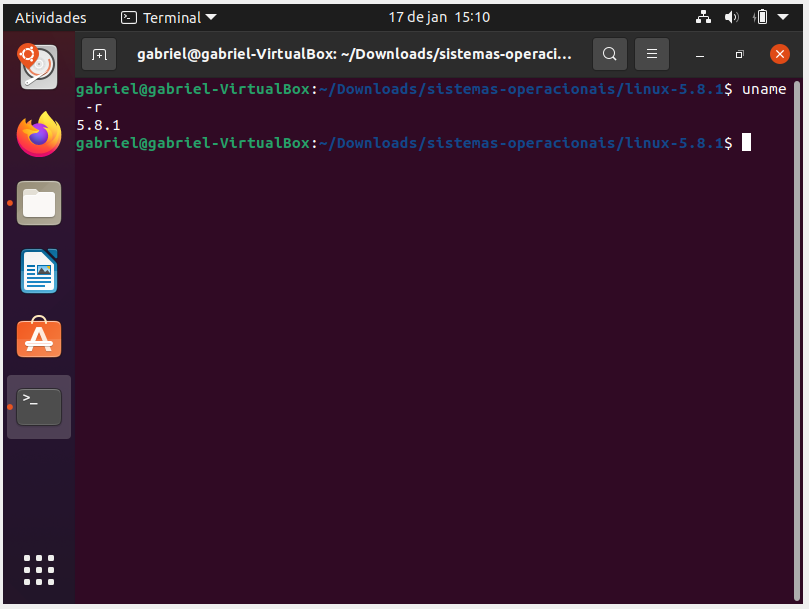
\includegraphics[width=12cm]{img/novo_kernel.png}
    \end{figure}
    
    \subsection{Teste para a chamada no kernel}
    
    \begin{figure}[hbp!]
        \centering
        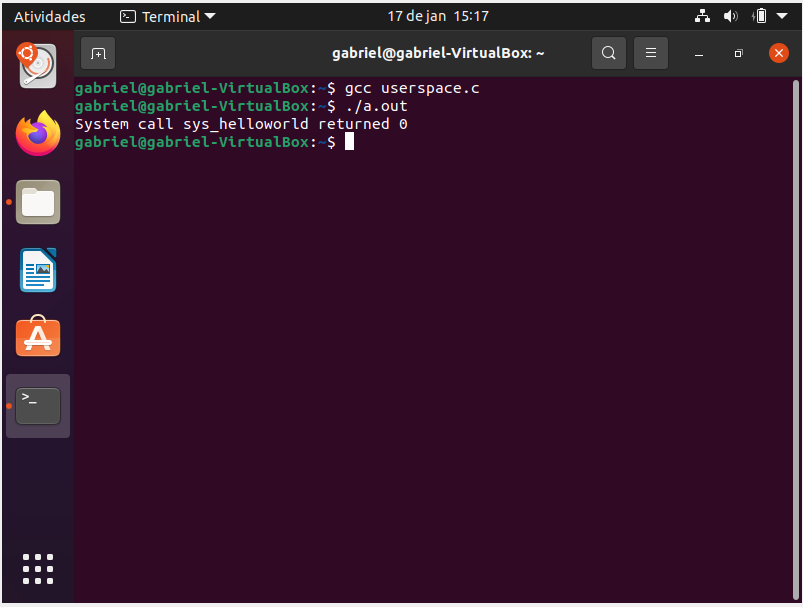
\includegraphics[width=12cm]{img/teste_chamada.png}
    \end{figure}
    
    \subsection{Mensagem no kernel}
    
    \begin{figure}[hbp!]
        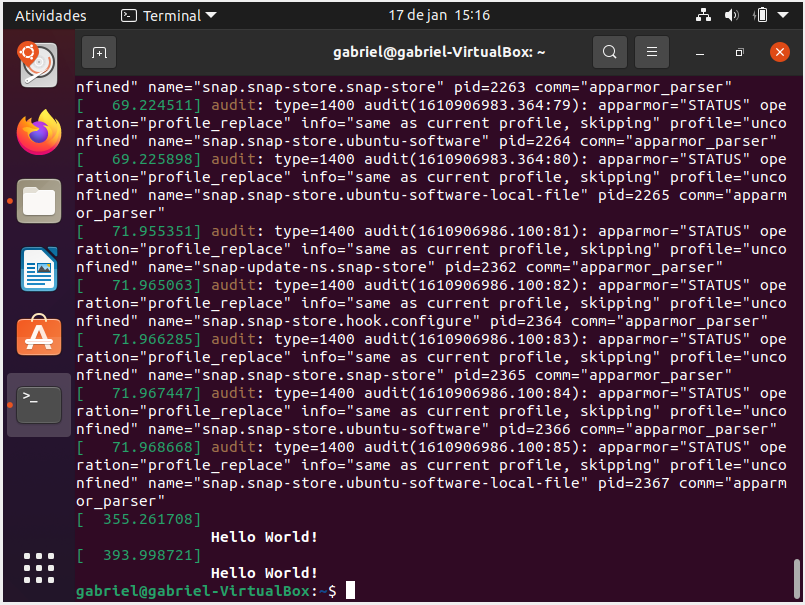
\includegraphics[width=12cm]{img/mensagem_kernel.png}
        \centering
    \end{figure}
	
\end{document}
